\documentclass[tikz,border=3pt]{standalone}
\usepackage[utf8]{inputenc}
\usepackage[T1]{fontenc}
\usepackage{lmodern}
\renewcommand{\familydefault}{\sfdefault}
\usepackage{sansmath}\sansmath
\usepackage{chemfig}
\usepackage{pgfplots}\pgfplotsset{compat=1.18,/pgf/number format/use comma,/pgf/number format/1000 sep={.}}
\usetikzlibrary{arrows.meta,calc,positioning,decorations.pathmorphing,patterns}
% paleta del sitio
\definecolor{nar}{HTML}{E8680C}\definecolor{narc}{HTML}{FFB35C}\definecolor{hielo}{HTML}{FFF3E8}
\definecolor{tinta}{HTML}{1D1D1F}\definecolor{gris}{HTML}{6E6E73}\definecolor{lila}{HTML}{7C5CF0}
\definecolor{azul}{HTML}{2F6FD6}\definecolor{menta}{HTML}{17A673}\definecolor{coral}{HTML}{E8342A}
\begin{document}
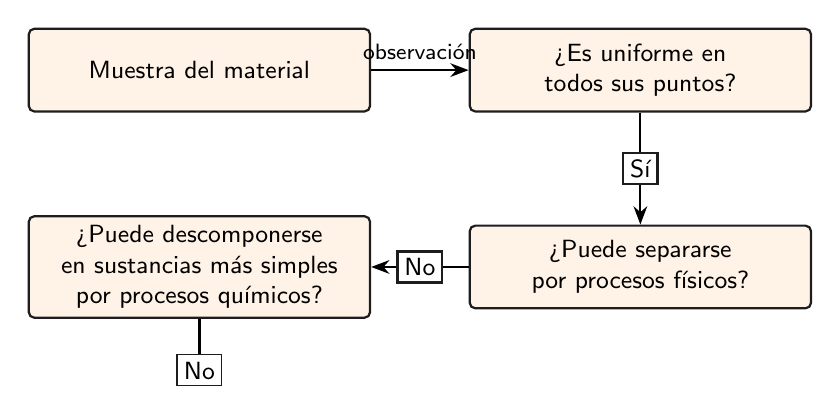
\begin{tikzpicture}[font=\small]

\tikzset{caja/.style={draw=tinta,thick,fill=hielo,rounded corners=2pt,align=center,text width=4.1cm,minimum height=1.05cm},
 resp/.style={draw=tinta,fill=white,inner sep=2.5pt}}
\node[caja] (m) at (0,0) {Muestra del material};
\node[caja] (u) at (5.6,0) {¿Es uniforme en\\todos sus puntos?};
\node[caja] (f) at (5.6,-2.5) {¿Puede separarse por procesos físicos?};
\node[caja] (q) at (0,-2.5) {¿Puede descomponerse en sustancias más simples por procesos químicos?};
\draw[-{Stealth},thick] (m) -- node[above,font=\footnotesize]{observación} (u);
\draw[-{Stealth},thick] (u) -- node[resp]{Sí} (f);
\draw[-{Stealth},thick] (f) -- node[resp]{No} (q);
\draw[thick] (q.south) -- ++(0,-0.45);
\node[resp,below] at ($(q.south)+(0,-0.45)$) {No};

\end{tikzpicture}
\end{document}
